% Dokumentenklasse
\documentclass[12pt,a4paper,oneside]{article}

% Pakete
% Schriftarten und Typografie
\usepackage{fontspec}  % Ermöglicht die Verwendung von TrueType/OpenType-Schriftarten mit XeLaTeX
\usepackage[T1]{fontenc} % Korrekte Darstellung von Umlauten und Sonderzeichen
\usepackage{textcomp}   % Zusätzliche Schriftzeichen wie Euro-Symbol
\usepackage{microtype}  % Optimiert die Mikrotypografie für bessere Lesbarkeit

% Hauptschriftart einstellen (Tex Gyre Termes, aber anpassbar)
\setmainfont[
    Path = /Users/jan/Library/Fonts/,  % Pfad zu den Schriftarten
    BoldFont = texgyretermes-bold.otf,
    ItalicFont = texgyretermes-italic.otf,
    BoldItalicFont = texgyretermes-bolditalic.otf
]{texgyretermes-regular.otf}

% Monospaced-Schriftart für Quellcode oder ähnliches
\setmonofont{Source Code Pro}


\usepackage[ngerman]{babel}   % Deutsche Sprachunterstützung
\usepackage[german=quotes]{csquotes}

\usepackage{amsmath} % Erweiterte mathematische Funktionalität
\usepackage{amssymb} % Zusätzliche mathematische Symbole
\usepackage{microtype} % Verbesserte Typografie
\usepackage{graphicx} % Für Grafiken
\usepackage{tikz}
\usetikzlibrary{mindmap, shapes, backgrounds}
\usepackage{setspace}
\usepackage[font=small,labelfont=bf]{caption}
\usepackage{subcaption} % Mehrere Unterbilder
\usepackage[left=2.5cm,right=2.5cm,top=2.5cm,bottom=2.5cm]{geometry}
\usepackage{url}

% Tabellen und Listen
\usepackage{booktabs}   % Hochwertige Tabellen
\usepackage{multirow}
\usepackage{makecell}
\usepackage{tabularx}   % Flexible Tabellen
\usepackage{enumitem}   % Anpassen von Aufzählungen und Listen
\setlist[enumerate,1]{label=\alph*)}
\setlist{itemsep=0pt}   % Kein Abstand zwischen Listenelementen

% Literaturverzeichnis
\usepackage[backend=biber, style=ieee, defernumbers=true]{biblatex}  % Verwendung von Biber als Backend und IEEE-Stil (kompatibel mit XeLaTeX)
\addbibresource{references.bib}  % Einbinden der Bibliographie-Datei
\ExecuteBibliographyOptions{backref=true,backrefstyle=three+,url=true,urldate=comp,abbreviate=false,maxbibnames=20}
\DeclareBibliographyCategory{cited}
\let\defaultcite\cite
\renewcommand*\cite[2][]{\addtocategory{cited}{#2}\defaultcite[#1]{#2}}

% Farben und Listings für Quellcode
\usepackage[dvipsnames,svgnames,x11names]{xcolor} % Erweiterte Farbunterstützung
% colors_settings.tex
\providecommand{\definecolor}{}
\definecolor{DodgerBlue4}{rgb}{0.06, 0.31, 0.55}
\definecolor{DarkOrange}{rgb}{1.0, 0.55, 0}
\definecolor{DarkSlateGray}{rgb}{0.18,0.31,0.31}
\definecolor{gray33}{rgb}{0.33,0.33,0.33}
\definecolor{meinblue}{RGB}{3, 78, 154} % #034E9A
\usepackage{listings}
% listing_settings.tex
\lstset{
    basicstyle=\ttfamily\small,  % Monospaced-Schriftart für Quellcode
    language=C++,  % Programmiersprache
    breaklines=true,  % Zeilenumbruch
    showspaces=false,  % Keine Leerzeichen anzeigen
    showstringspaces=false,  % Keine Leerzeichen in Strings anzeigen
    showtabs=false,  % Keine Tabs anzeigen
    tabsize=4,  % Tabulatorgröße
    captionpos=t,  % Position der Bildunterschrift
    breakatwhitespace=false,  % Zeilenumbruch bei Leerzeichen
    title=\lstname,  % Titel des Listings
    keywordstyle=\color{black},  % Stil für Schlüsselwörter
    commentstyle=\color{gray33},  % Stil für Kommentare
    stringstyle=\color{DarkOrange},  % Stil für Strings
    %morekeywords={std, cout, endl},  % Zusätzliche Schlüsselwörter
    identifierstyle=\bfseries\color{black},  % Stil für Identifikatoren
    floatplacement=htbp,
    abovecaptionskip=.5\baselineskip,
    belowcaptionskip=.5\baselineskip,
    upquote=true,
    literate={á}{{\'a}}1 {é}{{\'e}}1 {í}{{\'i}}1 {ó}{{\'o}}1 {ú}{{\'u}}1
                {Á}{{\'A}}1 {É}{{\'E}}1 {Í}{{\'I}}1 {Ó}{{\'O}}1 {Ú}{{\'U}}1
                {à}{{\`a}}1 {è}{{\`e}}1 {ì}{{\`i}}1 {ò}{{\`o}}1 {ù}{{\`u}}1
                {À}{{\`A}}1 {È}{{\'E}}1 {Ì}{{\`I}}1 {Ò}{{\`O}}1 {Ù}{{\`U}}1
                {ä}{{\"a}}1 {ë}{{\"e}}1 {ï}{{\"i}}1 {ö}{{\"o}}1 {ü}{{\"u}}1
                {Ä}{{\"A}}1 {Ë}{{\"E}}1 {Ï}{{\"I}}1 {Ö}{{\"O}}1 {Ü}{{\"U}}1
                {â}{{\^a}}1 {ê}{{\^e}}1 {î}{{\^i}}1 {ô}{{\^o}}1 {û}{{\^u}}1
                {Â}{{\^A}}1 {Ê}{{\^E}}1 {Î}{{\^I}}1 {Ô}{{\^O}}1 {Û}{{\^U}}1
                {œ}{{\oe}}1 {Œ}{{\OE}}1 {æ}{{\ae}}1 {Æ}{{\AE}}1 {ß}{{\ss}}1
                {ű}{{\H{u}}}1 {Ű}{{\H{U}}}1 {ő}{{\H{o}}}1 {Ő}{{\H{O}}}1
                {ç}{{\c c}}1 {Ç}{{\c C}}1 {ø}{{\o}}1 {å}{{\r a}}1 {Å}{{\r A}}1
                {€}{{\EUR}}1 {£}{{\pounds}}1 {~}{{\textasciitilde}}1 {-}{{-}}1
}
    

% Fußnoten
\usepackage{footnote}   % Verbesserte Fußnotenverwaltung
\usepackage{fnpct}      % Verwaltung der Fußnoten und Interaktion mit Satzzeichen
\setfnpct{after-punct-space={-.2em}}

% Globale Einstellung für alle Listen
\setlist{noitemsep, topsep=0pt}

% Formatierung
\onehalfspacing
\renewcommand{\normalsize}{\fontsize{12pt}{14pt}\selectfont}
\renewcommand{\large}{\fontsize{14pt}{17pt}\selectfont}

% Umbenennen der Verzeichnisse
\renewcommand{\listfigurename}{Abbildungen}
\renewcommand{\listtablename}{Tabellen}
\renewcommand{\refname}{Literatur}
\renewcommand{\figurename}{Abb.}
\renewcommand{\tablename}{Tab.}

% Hyperlinks und Querverweise
\usepackage[hidelinks]{hyperref}  % Versteckte Links (ohne Umrandung)
\usepackage[ngerman]{cleveref}    % Intelligente Querverweise
\hypersetup{
    colorlinks=true,
    linkcolor=meinblue,
    filecolor=meinblue,      
    urlcolor=meinblue,
    citecolor=meinblue, % Farbe für Literaturverweise
    pdftitle={Redaktionelles Feedback: LaTeX-Vorlage},
    pdfpagemode=FullScreen,
}

% Titelseite
\title{[Titel der Arbeit]}
\author{[Name des Autors]}
\date{13. Oktober 2024}

\begin{document}

% Titelseite ohne Seitenzahl
\begin{titlepage}
    \maketitle
    \thispagestyle{empty}
    
    % Abstract auf der Titelseite
    \begin{abstract}
        [Prägnante Zusammenfassung der Arbeit in 150-250 Wörtern. Enthält die Hauptfragestellung, den methodischen Ansatz, die wichtigsten Ergebnisse und die Schlussfolgerung.]
    \end{abstract}
\end{titlepage}
    
% Seitennummerierung beginnt mit römischen Zahlen
\pagenumbering{roman}

% Inhaltsverzeichnis
\tableofcontents
\clearpage

% Abbildungs- und Tabellenverzeichnis
\listoffigures
\listoftables
\clearpage

% Hauptteil beginnt hier, Seitennummerierung wechselt zu arabisch
\pagenumbering{arabic}

\section{Einleitung}
\subsection{Hintergrund und Motivation}
[Einführung in das Thema und Erläuterung seiner Relevanz. Beschreibung des aktuellen Forschungsstands und Identifikation von Forschungslücken.]

\subsection{Problemstellung und Zielsetzung}
[Klare Formulierung der Forschungsfrage(n) und der Ziele der Arbeit. Stellen Sie hier den roten Faden Ihrer Arbeit vor.]

\subsection{Aufbau der Arbeit}
[Überblick über die Struktur der folgenden Kapitel und deren Inhalte. Erklären Sie, wie die Kapitel aufeinander aufbauen und zum Erreichen des Forschungsziels beitragen.]

\clearpage
\section{Theoretische Grundlagen und Stand der Forschung}
\subsection{Zentrale Begriffe und Konzepte}
[Definition und Erläuterung der wichtigsten Begriffe und Konzepte. Verwenden Sie \textit{kursiv} für Fachbegriffe bei ihrer ersten Nennung.]

\subsection{Aktueller Forschungsstand}
[Überblick über den aktuellen Stand der Forschung im Themengebiet. Diskutieren Sie verschiedene Perspektiven und identifizieren Sie Forschungslücken.]

\subsection{Theoretischer Rahmen}
[Vorstellung und Begründung des theoretischen Rahmens Ihrer Arbeit.]

\clearpage
\section{Methodisches Vorgehen}
\subsection{Forschungsdesign}
[Beschreiben Sie das gewählte Forschungsdesign und begründen Sie Ihre Wahl. Diskutieren Sie Vor- und Nachteile.]

\subsection{Datenerhebung}
[Erläutern Sie die Methoden der Datenerhebung, z.B. Interviews, Fragebögen, Experimente. Begründen Sie Ihre Auswahl.]

\subsection{Datenanalyse}
[Beschreiben Sie die Verfahren zur Datenanalyse, z.B. statistische Methoden, qualitative Inhaltsanalyse. Erklären Sie, warum diese Methoden für Ihre Forschungsfrage geeignet sind.]

\subsection{Ethische Überlegungen und Datenschutz}
[Diskutieren Sie ethische Aspekte Ihrer Forschung und erläutern Sie Maßnahmen zum Datenschutz.]

\clearpage
\section{Empirische Untersuchung und Ergebnisse}
\subsection{Durchführung der Untersuchung}
[Beschreiben Sie detailliert, wie Sie Ihre Untersuchung durchgeführt haben.]

\subsection{Darstellung der Ergebnisse}
[Präsentation der Forschungsergebnisse, ggf. mit Tabellen oder Grafiken. Achten Sie auf eine klare und übersichtliche Darstellung.]

% Beispiel für eine Abbildung
\begin{figure}[htbp]
    \centering
    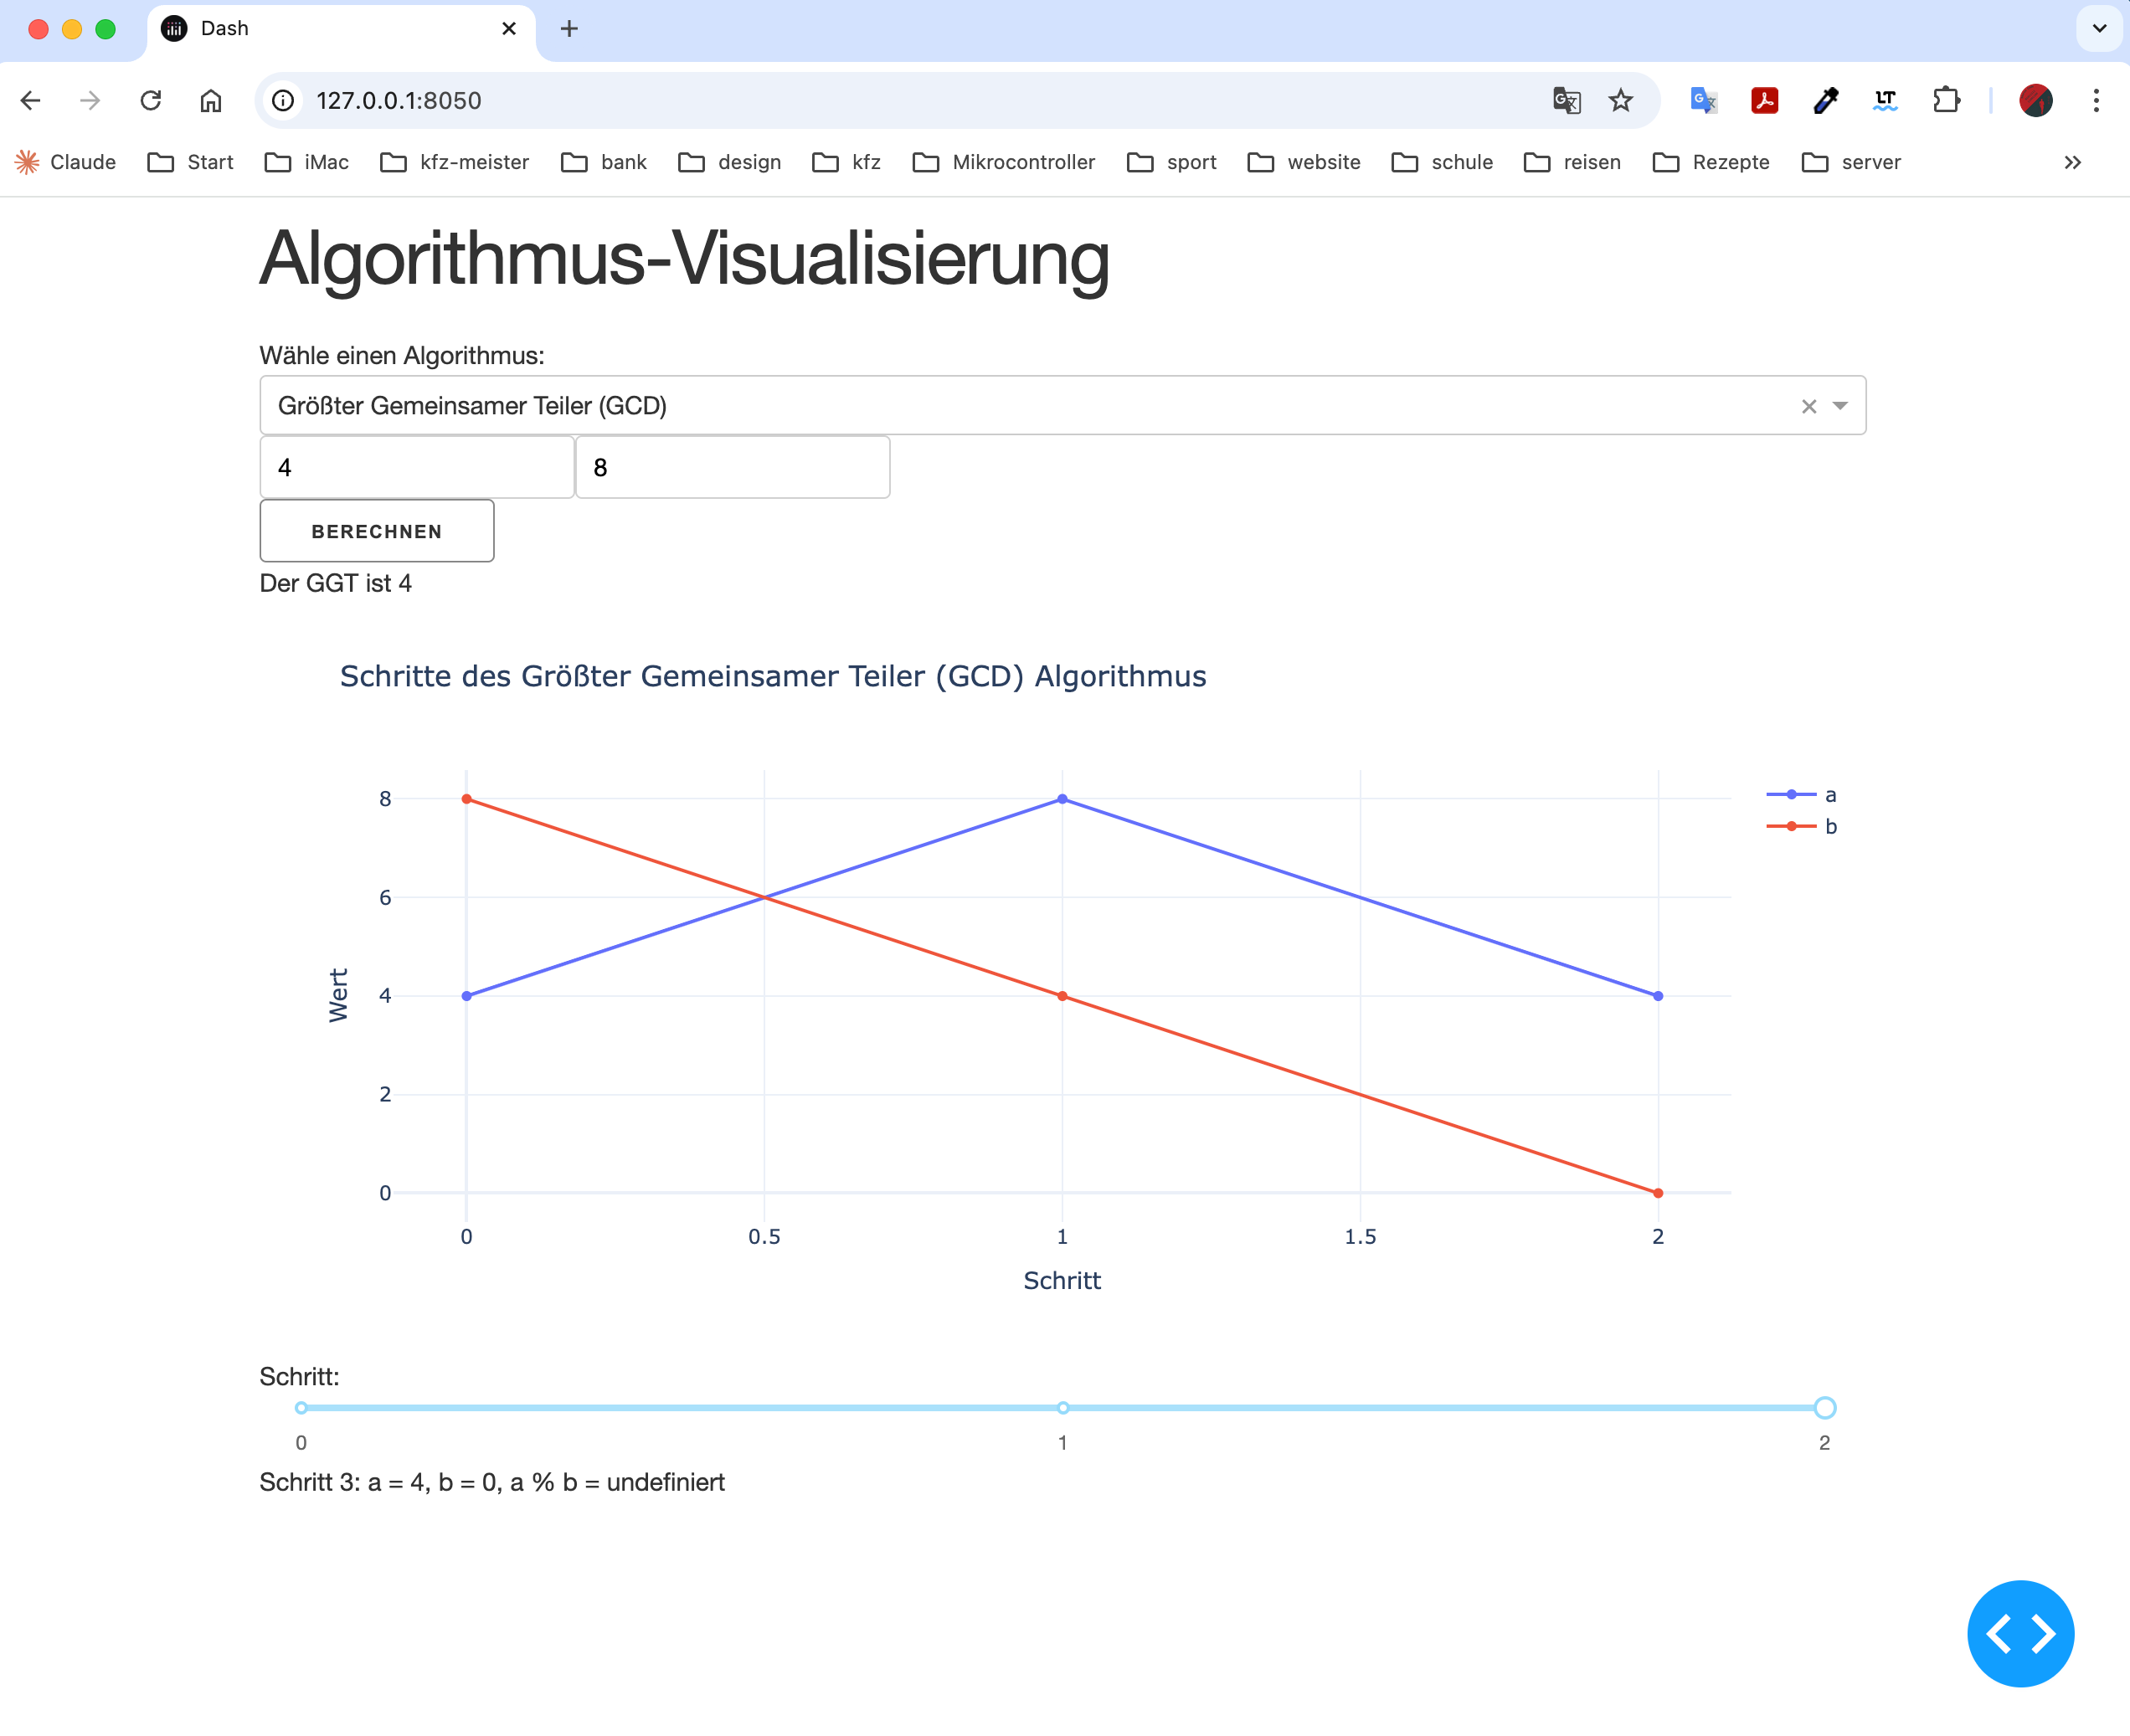
\includegraphics[width=0.8\textwidth]{images/ergebnisse_grafik.png}
    \caption{Visualisierung der Hauptergebnisse}
    \label{fig:ergebnisse}
\end{figure}

% Beispiel für eine Tabelle
\begin{table}[htbp]
    \centering
    \caption{Zusammenfassung der wichtigsten Ergebnisse}
    \label{tab:ergebnisse}
    \begin{tabularx}{\textwidth}{@{}lXX@{}}
    \toprule
    \textbf{Aspekt} & \textbf{Ergebnis} & \textbf{Interpretation} \\
    \midrule
    Aspekt 1 & Ergebnis 1 & Interpretation 1 \\
    Aspekt 2 & Ergebnis 2 & Interpretation 2 \\
    \bottomrule
    \end{tabularx}
\end{table}

\clearpage
\section{Diskussion und Interpretation}
\subsection{Interpretation der Ergebnisse}
[Interpretieren Sie Ihre Ergebnisse im Kontext Ihrer Forschungsfrage und des theoretischen Rahmens.]

\subsection{Vergleich mit bisherigen Forschungsergebnissen}
[Setzen Sie Ihre Ergebnisse in Beziehung zu bisherigen Forschungsarbeiten. Diskutieren Sie Übereinstimmungen und Abweichungen.]

\subsection{Kritische Reflexion der Methodik}
[Reflektieren Sie kritisch über die Stärken und Schwächen Ihrer methodischen Vorgehensweise.]

\clearpage
\section{Schlussfolgerung und Ausblick}
\subsection{Zusammenfassung der Hauptergebnisse}
[Fassen Sie die wichtigsten Erkenntnisse Ihrer Arbeit prägnant zusammen.]

\subsection{Beantwortung der Forschungsfrage}
[Beantworten Sie explizit die in der Einleitung gestellte(n) Forschungsfrage(n).]

\subsection{Limitationen der Arbeit}
[Diskutieren Sie offen die Grenzen und möglichen Schwächen Ihrer Untersuchung.]

\subsection{Ausblick auf zukünftige Forschung}
[Skizzieren Sie Ansätze für weiterführende Forschung und offene Fragen, die sich aus Ihrer Arbeit ergeben.]

\subsection{Praktische Implikationen}
[Erläutern Sie die praktische Relevanz Ihrer Forschungsergebnisse. Geben Sie konkrete Handlungsempfehlungen, wenn möglich.]

\clearpage
\section{Interdisziplinäre Perspektiven}
[Diskutieren Sie, wie Ihre Forschung mit anderen Fachgebieten in Verbindung steht und welche fachübergreifenden Erkenntnisse gewonnen werden können. Zeigen Sie Verbindungen und mögliche Synergien auf.]

% Literaturverzeichnis
\clearpage
\printbibliography[title=Literaturverzeichnis]
\addcontentsline{toc}{section}{Literaturverzeichnis}

% Anhang
\clearpage
\appendix
\section{Anhang}
\subsection{Detaillierte Berechnungen}
[Fügen Sie hier detaillierte Berechnungen ein, die im Hauptteil zu umfangreich wären.]

\subsection{Interviewleitfaden und Transkripte}
[Fügen Sie hier den verwendeten Interviewleitfaden und anonymisierte Transkripte von durchgeführten Interviews ein.]

\subsection{Ergänzende Statistiken und Daten}
[Präsentieren Sie hier zusätzliche statistische Auswertungen und Rohdaten, die im Hauptteil nicht Platz fanden.]

\clearpage
% Eidesstattliche Erklärung
\section*{Eidesstattliche Erklärung}
%\addcontentsline{toc}{section}{Eidesstattliche Erklärung}
Ich erkläre hiermit an Eides statt, dass ich die vorliegende Arbeit selbstständig und ohne Benutzung anderer als der angegebenen Hilfsmittel angefertigt habe. Die aus fremden Quellen direkt oder indirekt übernommenen Gedanken sind als solche kenntlich gemacht.

\vspace{2cm}
\noindent
\makebox[6cm]{\hrulefill} \hfill \makebox[6cm]{\hrulefill}\\
Ort, Datum \hfill Unterschrift

\end{document}